\documentclass{article}%
\usepackage{amsmath}%
\usepackage{amsfonts}%
\usepackage{amssymb}%
\usepackage{graphicx}
\usepackage[export]{adjustbox}
\usepackage{enumitem}
\usepackage{multirow}
\usepackage[usenames, dvipsnames]{xcolor}
\usepackage[export]{adjustbox}
\usepackage{subcaption}
\usepackage[T1]{fontenc}
\usepackage{hyperref}
%-------------------------------------------
\newtheorem{theorem}{Theorem}
\newtheorem{acknowledgement}[theorem]{Acknowledgement}
\newtheorem{algorithm}[theorem]{Algorithm}
\newtheorem{axiom}[theorem]{Axiom}
\newtheorem{case}[theorem]{Case}
\newtheorem{claim}[theorem]{Claim}
\newtheorem{conclusion}[theorem]{Conclusion}
\newtheorem{condition}[theorem]{Condition}
\newtheorem{conjecture}[theorem]{Conjecture}
\newtheorem{corollary}[theorem]{Corollary}
\newtheorem{criterion}[theorem]{Criterion}
\newtheorem{definition}[theorem]{Definition}
\newtheorem{example}[theorem]{Example}
\newtheorem{exercise}[theorem]{Exercise}
\newtheorem{lemma}[theorem]{Lemma}
\newtheorem{notation}[theorem]{Notation}
\newtheorem{problem}[theorem]{Problem}
\newtheorem{proposition}[theorem]{Proposition}
\newtheorem{remark}[theorem]{Remark}
\newtheorem{solution}[theorem]{Solution}
\newtheorem{summary}[theorem]{Summary}
\newenvironment{proof}[1][Proof]{\textbf{#1.} }{\ \rule{0.5em}{0.5em}}
\setlength{\textwidth}{7.0in}
\setlength{\oddsidemargin}{-0.35in}
\setlength{\topmargin}{-0.5in}
\setlength{\textheight}{9.0in}
\setlength{\parindent}{0.3in}
\begin{document}

\begin{flushright}
\textbf{Chanjoon Park \\
Feb 11, 2024}
\end{flushright}

\begin{center}
\textbf{CS 285: Deep Reinforcement Learning, Decision Making, and Control \\
Assignment 1. Imitation Learning \\}
\end{center}

\section*{3. Behavioral Cloning}

\subsection*{1. Run BC and report results}

\begin{table}[h!]
	\centering
	\begin{tabular}{ |c||c|c|c|c|c|  }
	\hline
	\textbf{Gym Env}&Avg. Return&Std. Return&Eval batch size&Episode&Expert's Avg. Return\\
	\hline
	\textbf{Ant-v4}& 1153.34& 142.75&  5000&1000&4681.89\\
	\textbf{HalfCheetah-v4}&3293.29& 150.43&5000&1000&4034.80\\
	\textbf{Hopper-v4}&1106.97& 417.64&5000&1000&3717.51\\
	\textbf{Walker2d-v4}&406.20& 431.96&5000&1000&5383.31\\
	\hline
 \end{tabular}
 \caption{The mean and standard deviation of trained policy with given parameters.}
 \label{Table:1}
\end{table}

Above results are collected from approximately 5 trajectories as you can see in \textsc{\textrm{Eval batch size}} and \textsc{\textrm{Episode}} and only the HalfCheetah-v4 environment shows at least 30\% performance compared to the expert's policy.(Actually, 81.62\% achieved.) The other environments show less than 30\% performance, 24.63\%, 29.78\%, and 7.55\% for Ant-v4, Hopper-v4, and Walker2d-v4, respectively.

\subsection*{2. Experiment with one set of hyperparameters.}

\begin{figure}[!h]
	\centering
	\begin{subfigure}{0.48\textwidth}
		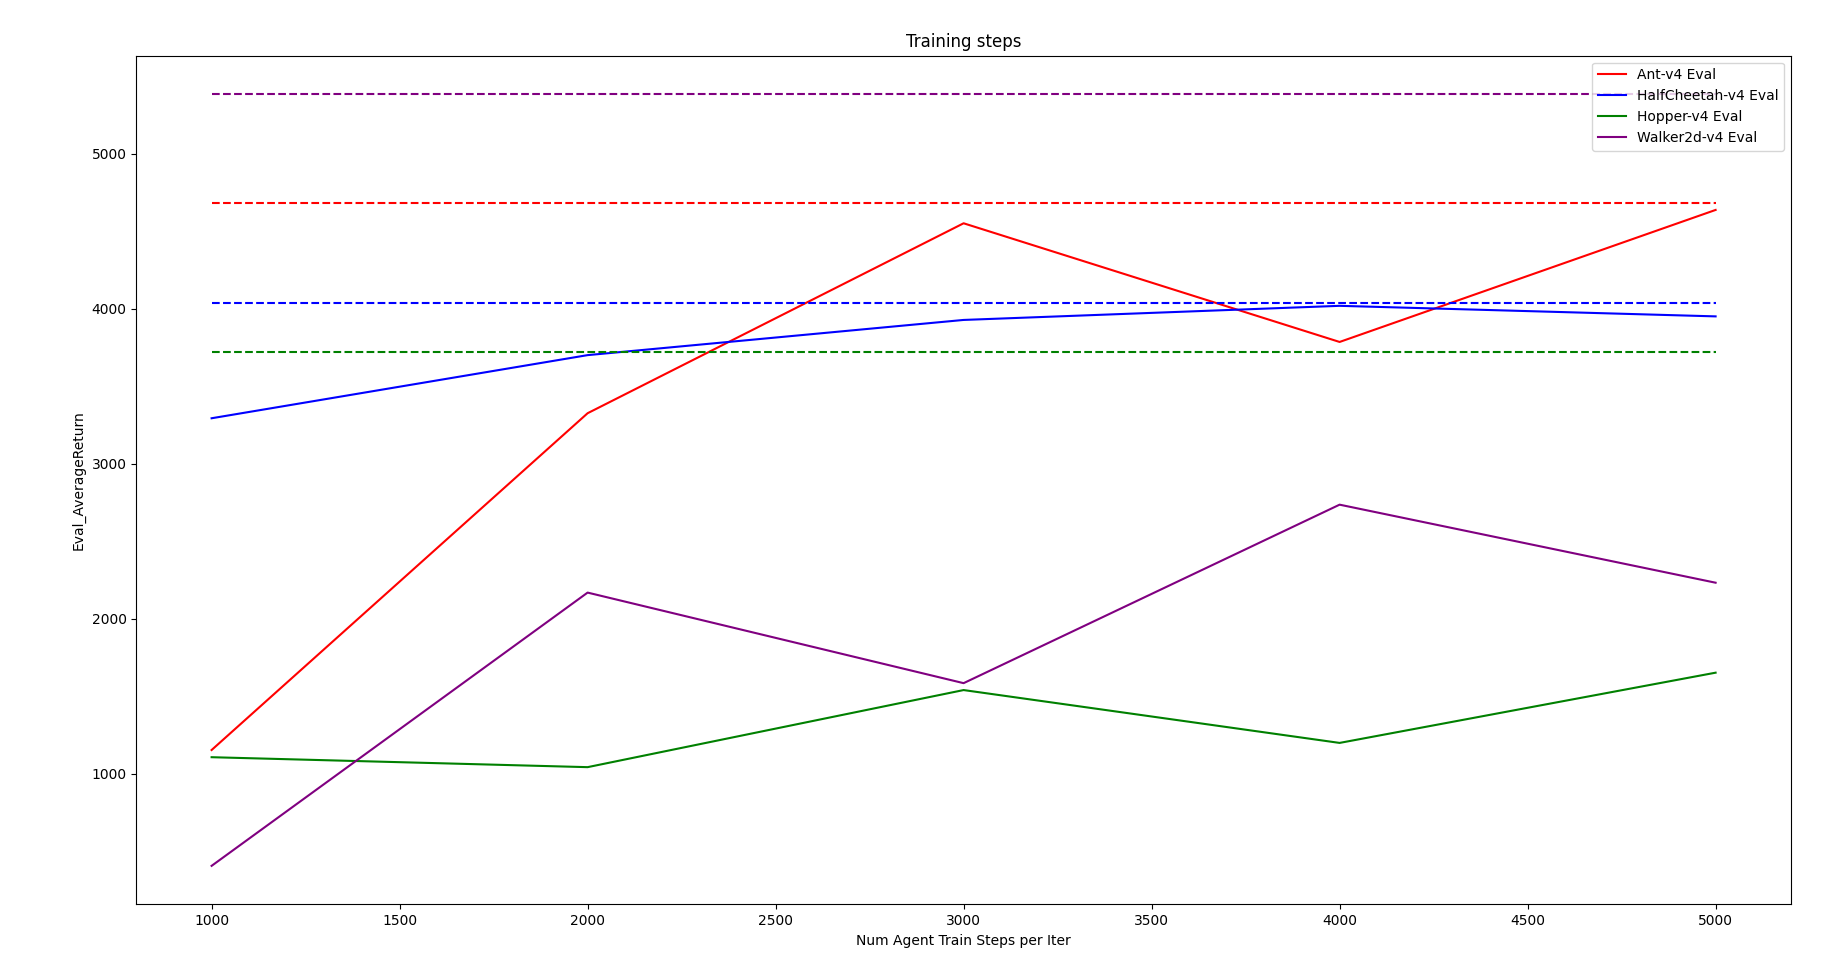
\includegraphics[width=0.9\linewidth, left]{hw1_3_training_steps.png} 
		\caption{Training steps}
		\label{fig:1}
	\end{subfigure}
	\begin{subfigure}{0.48\textwidth}
		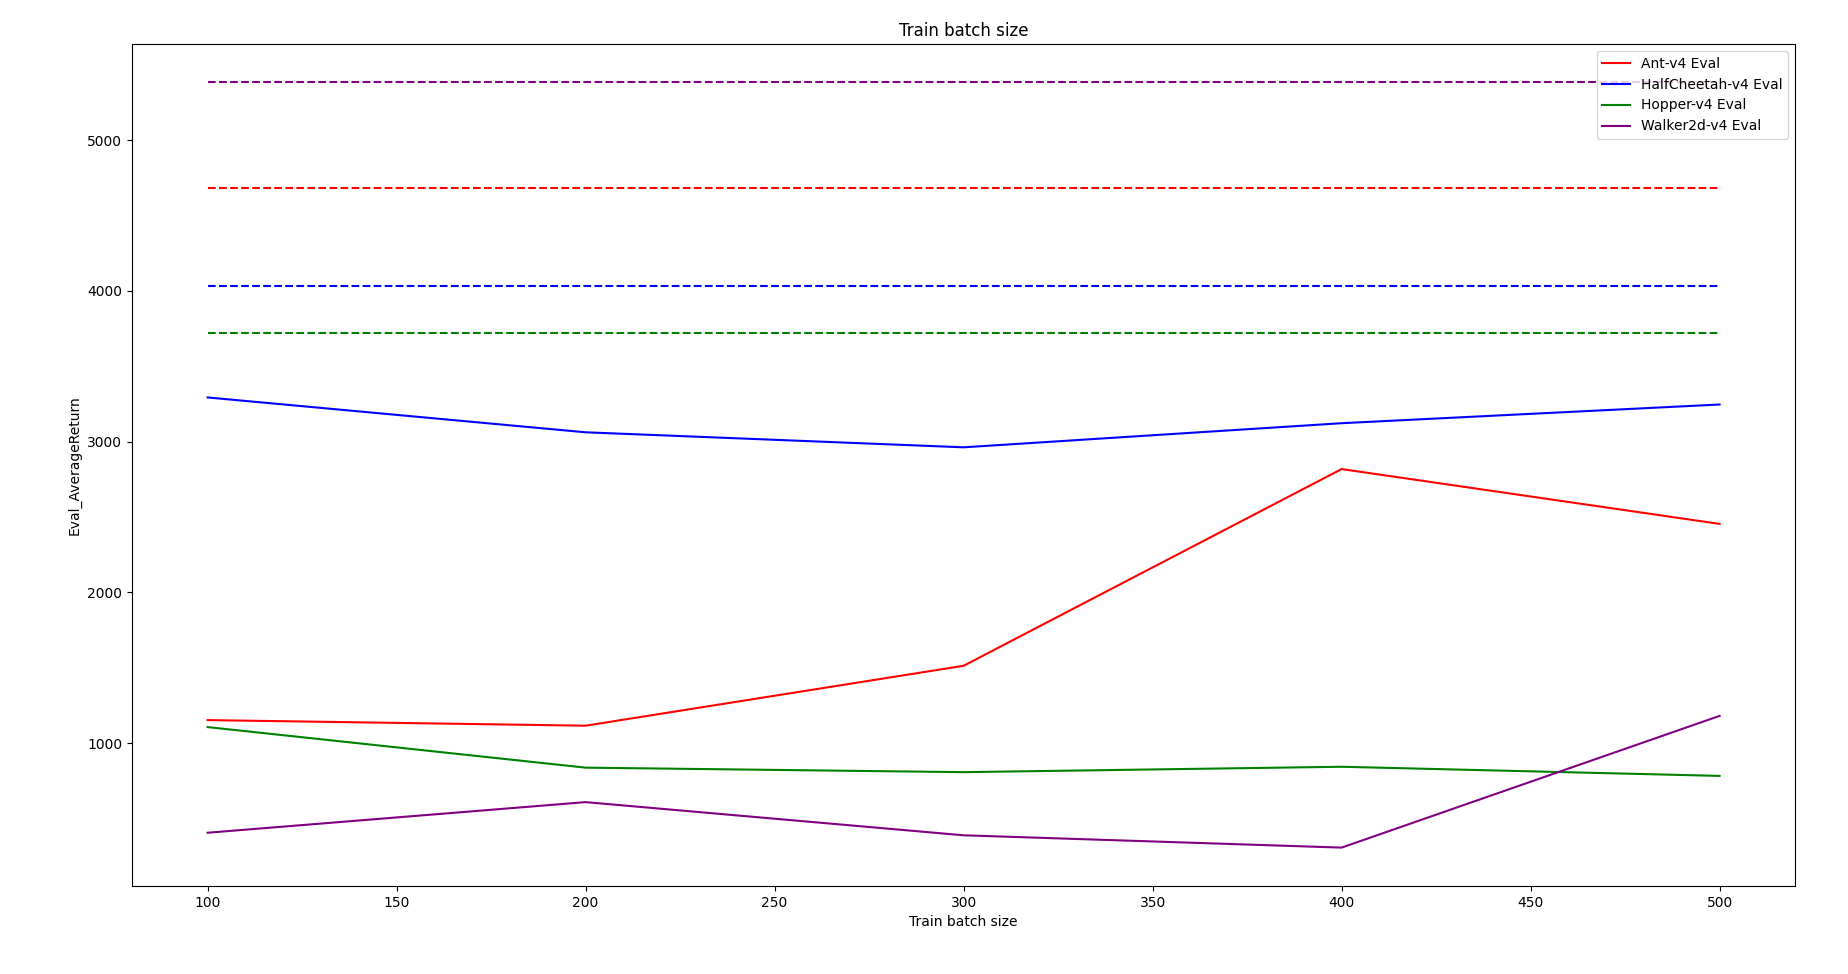
\includegraphics[width=0.9\linewidth, right]{hw1_3_train_batch_size.png}
		\caption{Batch size}
		\label{fig:2}
	\end{subfigure}
	\caption{The performance of the trained policy with different hyperparameters. \textcolor{red}{Red}, \textcolor{blue}{blue}, \textcolor{green}{green} and \textcolor{purple}{purple} line represents the Ant-v4, HalfCheetah-v4, Hopper-v4, and Walker2d-v4 environments, respectively and dotted line represents the expert's policy.}
\end{figure}

As we can see from the Figure \ref{fig:1}, the larger the training steps, the better the performance in general. However, the performance is not always improved as the training steps increase. For example, the performance of the Hopper-v4 and Walker2d-v4 environments is not improved as the training steps increase.

\vspace{12pt}

In the Figure \ref{fig:2}, there is no specific pattern that the performance is improved as the batch size increases.

\newpage
\section*{4. \textsc{DAgger}}

\begin{figure}[h]
	\centering
	\begin{subfigure}{0.48\textwidth}
			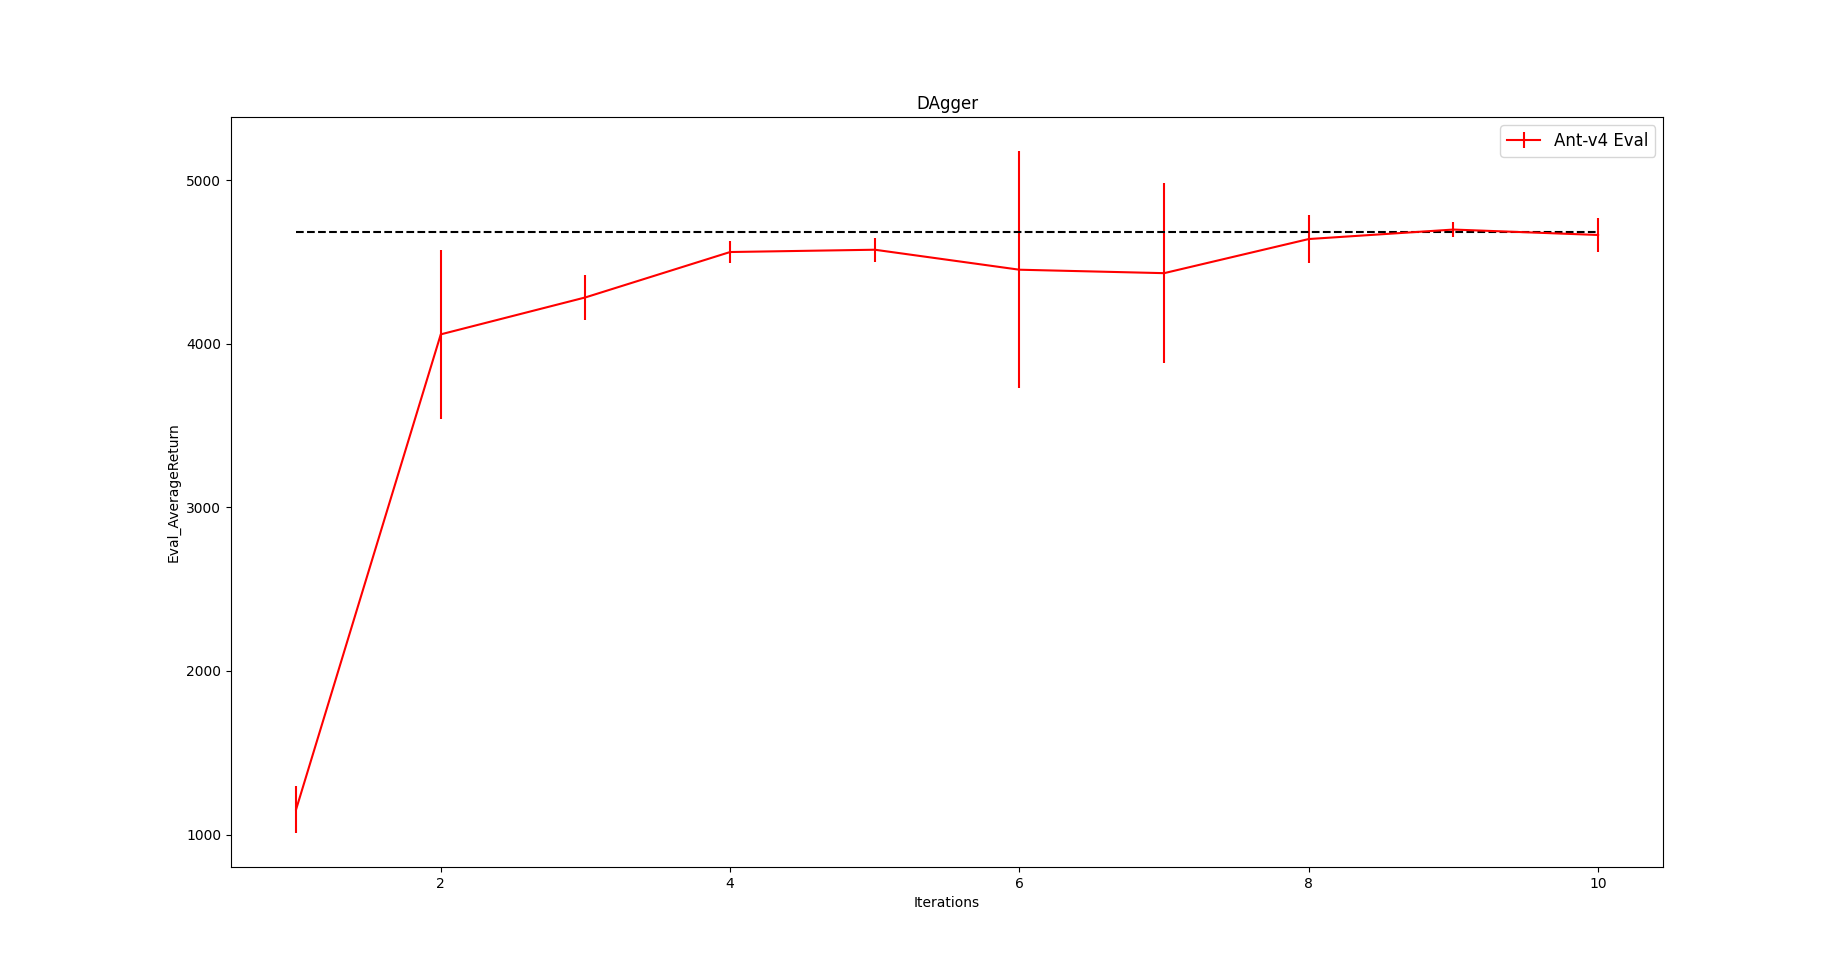
\includegraphics[width=\textwidth]{hw1_4_ant-v4.png}
			\subcaption{And-v4.}
	\end{subfigure}
	\begin{subfigure}{0.48\textwidth}
			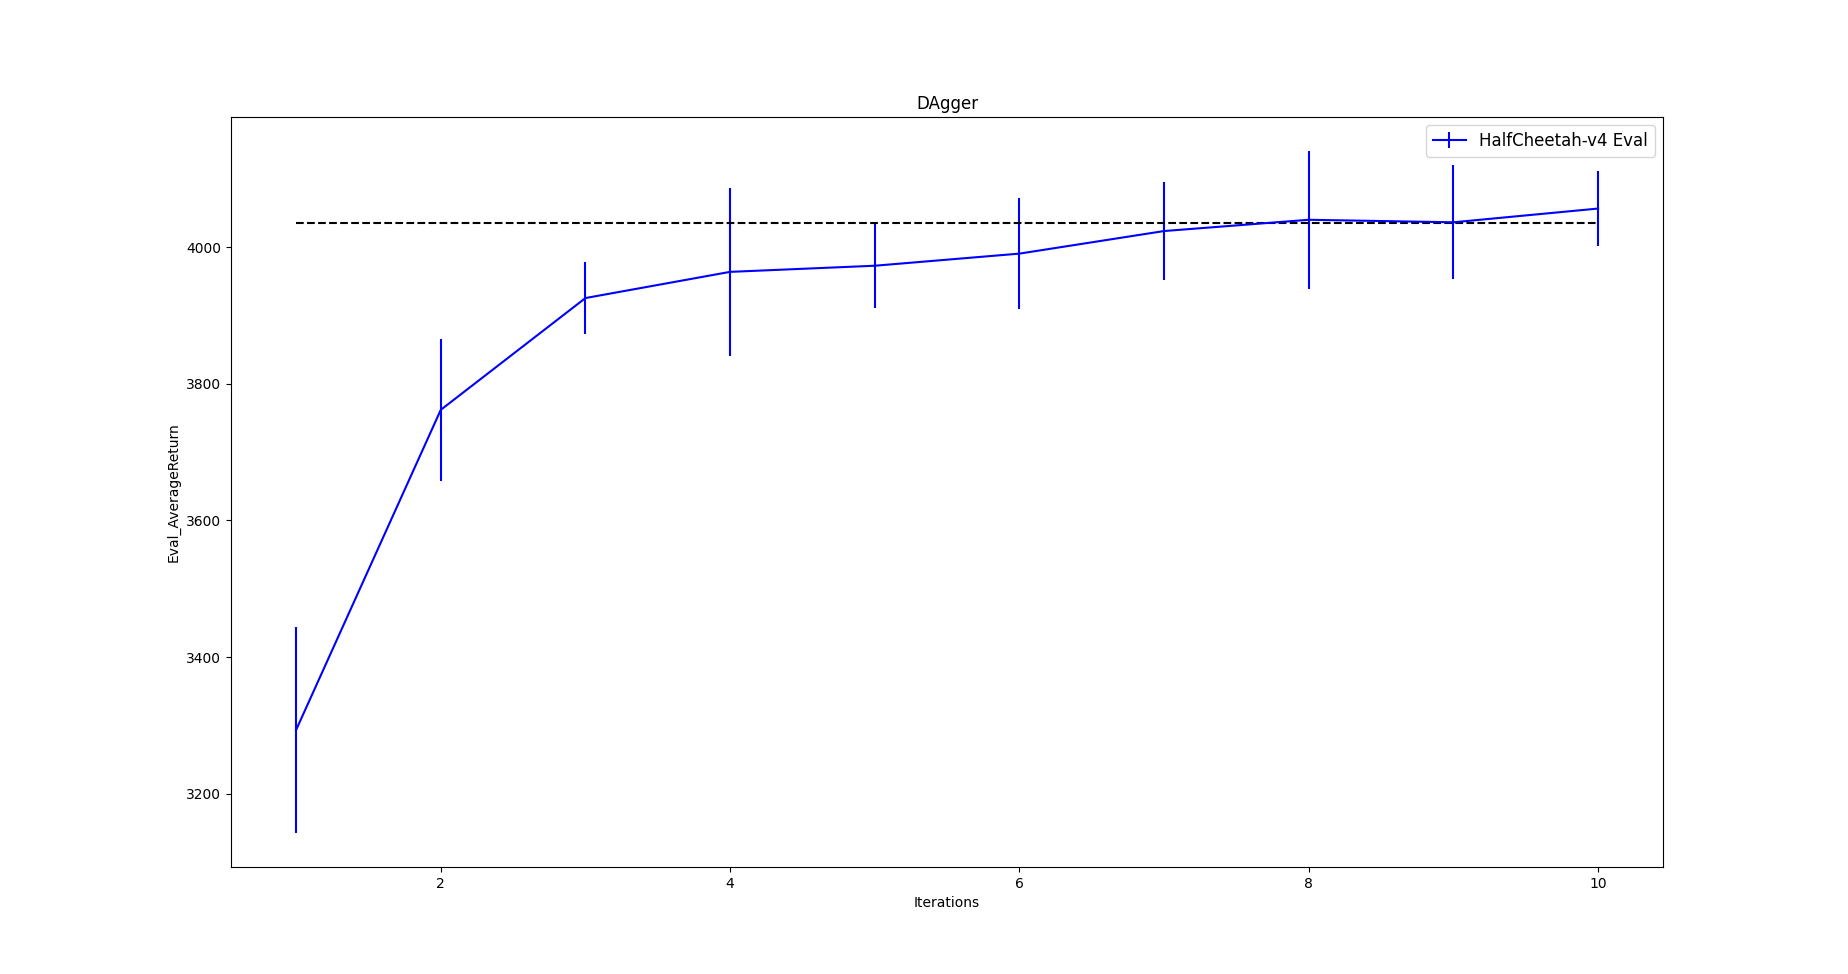
\includegraphics[width=\textwidth]{hw1_4_halfcheetah-v4.png}
			\subcaption{HalfCheetah-v4.}
	\end{subfigure}
	\\
	\begin{subfigure}{0.48\textwidth}
			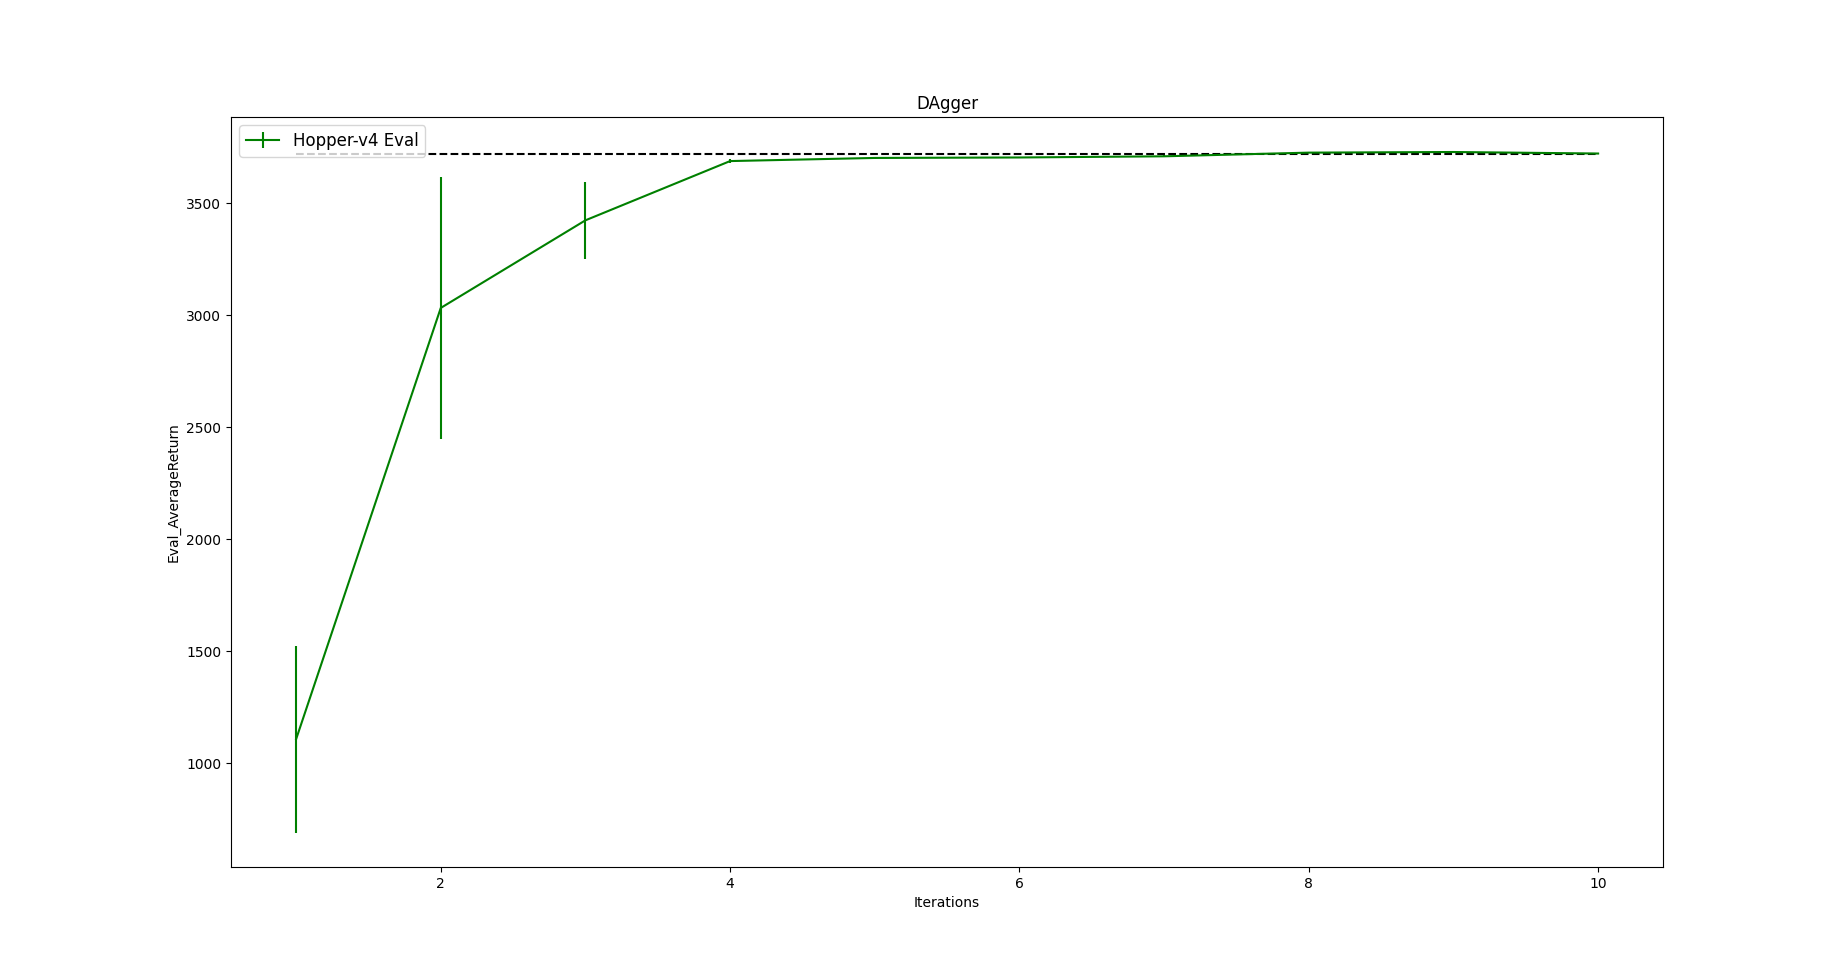
\includegraphics[width=\textwidth]{hw1_4_hopper-v4.png}
			\subcaption{Hopper-v4.}
	\end{subfigure}
	%
	\begin{subfigure}{0.48\textwidth}
			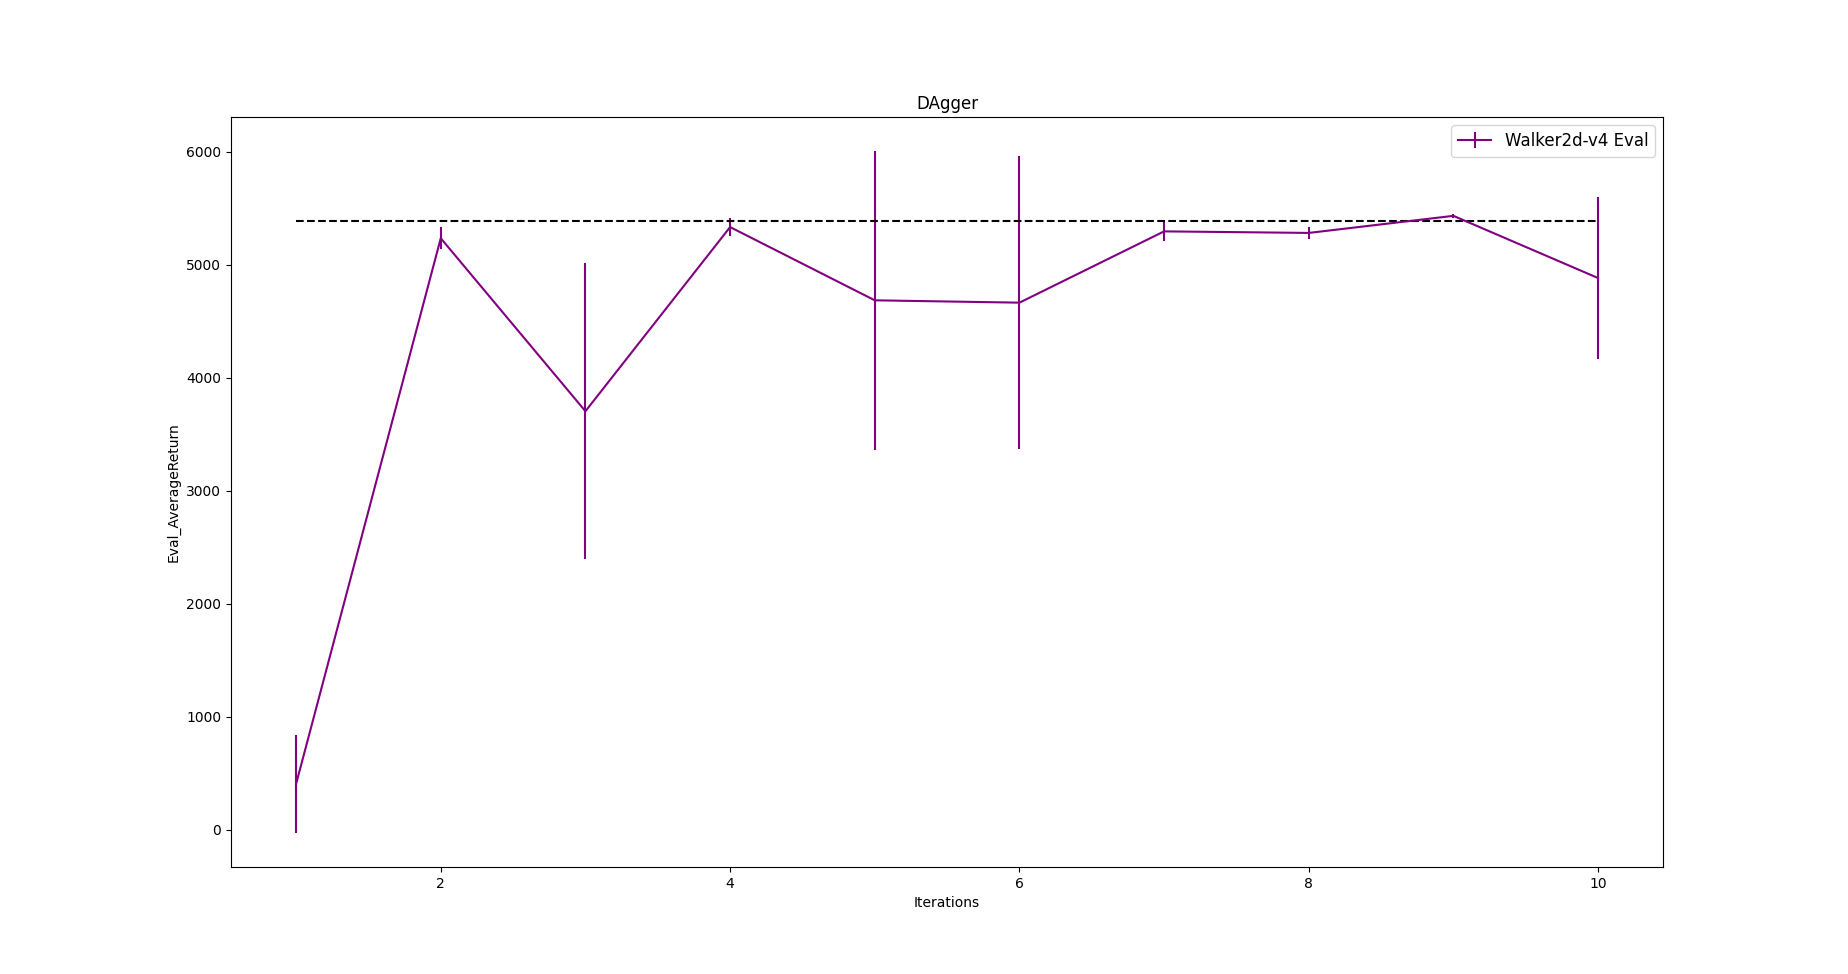
\includegraphics[width=\textwidth]{hw1_4_walker2d-v4.png}
			\subcaption{Walker2d-v4.}
	\end{subfigure}
	\caption{The performance of the trained policy with DAgger for each environment. Black dotted line represents the expert's policy.}
\end{figure}

DAgger improves the performance of the trained policy over iterations. The performance of the trained policy is improved as the number of iterations increases generally. 

\paragraph*{Note}
\textit{the commands to run the code are listed in the }\href{https://github.com/ChanJoon/CS285_hw_fall2023/tree/main/hw1/README.md}{README.md}

\end{document}
% https://www.overleaf.com/latex/templates/computer-science-homework-template/cktrjmbzsqpt